\documentclass{article}
\usepackage{tikz}
\usepackage{amsmath}
% \usepackage[top=2cm, left=2.5cm, right=2.5cm, bottom=2.5cm]{geometry}

\begin{document}

\section*{Einführung}
Lass uns die Erkundung der Zahlensysteme mit dem uns bekannten 10-er System beschreiben. Betrachten wir die Zahl \textbf{1976}. Wir zeichnen einen Rahmen um die einzelnen Zahlen, damit wir die Stellen der Zahlen besser unterscheiden können.

\begin{center}
$1976 = $
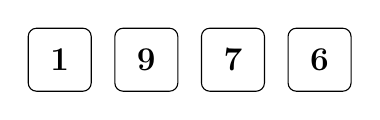
\begin{tikzpicture}[baseline=-0.5ex, every node/.style={align=center}]
    \foreach \digit [count=\i from 0] in {1, 9, 7, 6} {
        \node[draw, minimum width=0.8cm, minimum height=0.8cm, rounded corners=3pt] (tub\i) at (\i*1.1, 0) {\large $\mathbf{\digit}$};
    }
\end{tikzpicture}
\end{center}

Nun schreiben wir unter die einzelnen Zahlen die 10-er Potenzen:

\begin{center}
$1976 = $
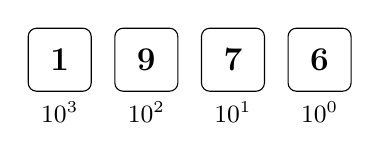
\begin{tikzpicture}[baseline=-0.5ex, every node/.style={align=center}]
    \foreach \digit/\power [count=\i from 0] in {1/10^3, 9/10^2, 7/10^1, 6/10^0} {
        \node[draw, minimum width=0.8cm, minimum height=0.8cm, rounded corners=3pt] (tub\i) at (\i*1.1, 0) {\large $\mathbf{\digit}$};
        \node[anchor=north, font=\small] at (tub\i.south) {$\power$};
    }
\end{tikzpicture}
\end{center}

Jetzt schreiben wir darunter das Produkt der Ziffern mit den 10-er Potenzen und summieren diese:

\begin{center}
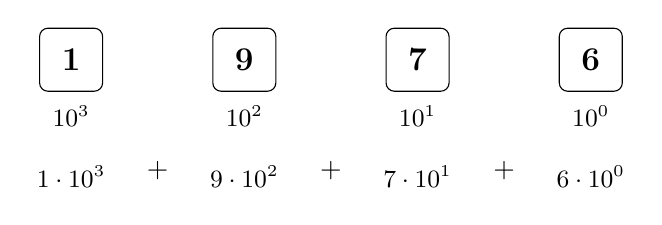
\begin{tikzpicture}[baseline=(box0.base), every node/.style={align=center}]
    \foreach \digit/\power/\prod [count=\i from 0] in {
        1 / 10^3 / 1 \cdot 10^3,
        9 / 10^2 / 9 \cdot 10^2,
        7 / 10^1 / 7 \cdot 10^1,
        6 / 10^0 / 6 \cdot 10^0
    } {
        \pgfmathsetmacro{\xpos}{\i*2.2}
        \node[draw, minimum width=0.8cm, minimum height=0.8cm, rounded corners=3pt] (box\i) at (\xpos, 0) {\large $\mathbf{\digit}$};
        \node[anchor=north, font=\small] (pow\i) at ([yshift=-0.05cm]box\i.south) {$\power$};
        \node[anchor=north, font=\small] (prod\i) at ([yshift=-0.25cm]pow\i.south) {$\prod$};
        \ifnum\i<3
            \node[anchor=base] at ({\xpos + 1.1}, {-0.8 - 0.7}) {$+$};
        \fi
    }
\end{tikzpicture}
\end{center}

Zum Schluss rechnen wir das Ganze aus:

\begin{center}
\begin{align*}
  &\phantom{= } 1 \cdot 10^3 + 9 \cdot 10^2 + 7 \cdot 10^1 + 6 \cdot 10^0 \\
  &= 1 \cdot 1000 + 9 \cdot 100 + 7 \cdot 10 + 6 \cdot 1 \\
  &= 1000 + 900 + 70 + 6 \\
  &= 1976
\end{align*}
\end{center}
Wir haben im 10-er System also die Ziffern 0, 1, 2, 3, 4, 5, 6, 7, 8 und 9.
\newpage

Schauen wir uns als nächstes eine größere Zahl an, zum Beispiel \textbf{8305710}. Auch hier wenden wir exakt dasselbe Prinzip an:

\begin{center}
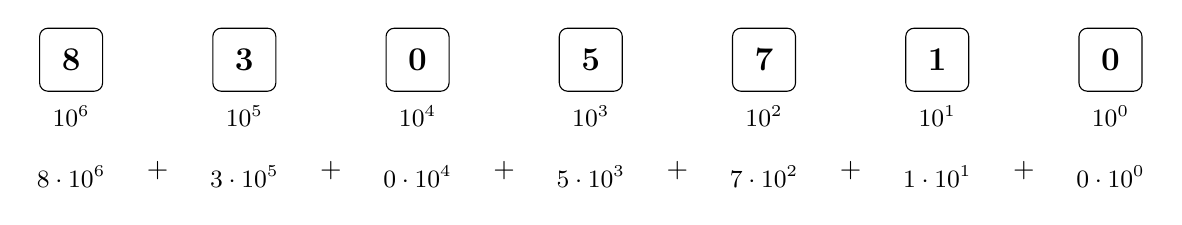
\begin{tikzpicture}[baseline=(box0.base), every node/.style={align=center}]
    % Schleife für die 7 Spalten der Zahl 8305710 (Ziffer / Potenz / Produkt)
    \foreach \digit/\power/\prod [count=\i from 0] in {
        8 / 10^6 / 8 \cdot 10^6,
        3 / 10^5 / 3 \cdot 10^5,
        0 / 10^4 / 0 \cdot 10^4,
        5 / 10^3 / 5 \cdot 10^3,
        7 / 10^2 / 7 \cdot 10^2,
        1 / 10^1 / 1 \cdot 10^1,
        0 / 10^0 / 0 \cdot 10^0
    } {
        % X-Position für jede Spalte berechnen (Abstand 2.2cm)
        \pgfmathsetmacro{\xpos}{\i*2.2}

        % 1. Zeile: Die Wanne mit der Ziffer darin
        \node[draw, minimum width=0.8cm, minimum height=0.8cm, rounded corners=3pt] (box\i) at (\xpos, 0) {\large $\mathbf{\digit}$};

        % 2. Zeile: Die Zehnerpotenz direkt darunter
        \node[anchor=north, font=\small] (pow\i) at ([yshift=-0.05cm]box\i.south) {$\power$};

        % 3. Zeile: Das Produkt direkt unter der Potenz
        \node[anchor=north, font=\small] (prod\i) at ([yshift=-0.25cm]pow\i.south) {$\prod$};

        % Pluszeichen in den Lücken zwischen den Produkten (bis zum vorletzten Element, hier i < 6)
        \ifnum\i<6
            \node[anchor=base] at ({\xpos + 1.1}, {-0.8 - 0.7}) {$+$};
        \fi
    }
\end{tikzpicture}
\end{center}

Zum Schluss rechnen wir das Ganze aus:

\begin{center}
\begin{align*}
  &\phantom{= } 8 \cdot 10^6 + 3 \cdot 10^5 + 0 \cdot 10^4 + 5 \cdot 10^3 + 7 \cdot 10^2 + 1 \cdot 10^1 + 0 \cdot 10^0 \\
  &= 8 \cdot 1000000 + 3 \cdot 100000 + 0 \cdot 10000 + 5 \cdot 1000 + 7 \cdot 100 + 1 \cdot 10 + 0 \cdot 1 \\
  &= 8000000 + 300000 + 0 + 5000 + 700 + 10 + 0 \\
  &= 8305710
\end{align*}
\end{center}

\section*{Übung: Stellenwerte bestimmen}
Versuche nun, die Zahl \textbf{1971} in das Schema einzutragen und die fehlenden Potenzen und Produkte zu ergänzen.

\vspace{0.5cm}

\begin{center}
\begin{tikzpicture}[baseline=(box0.base), every node/.style={align=center}]
    % Schleife für die 4 Spalten (mit Platzhaltern zum Ausfüllen)
    \foreach \i in {0, 1, 2, 3} {
        % X-Position für jede Spalte berechnen (Abstand 2.2cm)
        \pgfmathsetmacro{\xpos}{\i*2.2}

        % 1. Zeile: Leere Wanne (hier trägt man die Ziffer ein)
        \node[draw, minimum width=0.8cm, minimum height=0.8cm, rounded corners=3pt] (box\i) at (\xpos, 0) {};

        % 2. Zeile: Platzhalter für die Zehnerpotenz
        \node[anchor=north, font=\small] (pow\i) at ([yshift=-0.05cm]box\i.south) {$\dots$};

        % 3. Zeile: Platzhalter für das Produkt
        \node[anchor=north, font=\small] (prod\i) at ([yshift=-0.25cm]pow\i.south) {$\dots$};

        % Pluszeichen in den Lücken zwischen den Produkten (nur bis zum vorletzten Element)
        \ifnum\i<3
            \node[anchor=base] at ({\xpos + 1.1}, {-0.8 - 0.7}) {$+$};
        \fi
    }
\end{tikzpicture}
\end{center}

\vspace{0.8cm}
Berechne nun das Endergebnis:
\begin{center}
\begin{align*}
  &\phantom{= } \dots \cdot 10^3 + \dots \cdot 10^2 + \dots \cdot 10^1 + \dots \cdot 10^0 \\
  &= \dots + \dots + \dots + \dots \\
  &= \underline{\hspace{3cm}}
\end{align*}
\end{center}

\newpage

\section{Das 2-er System}
Das 2-er System nennt man auch das binaersystem. Sie hat nur die beiden Ziffern 0 und 1. Statt der 10-er Potenzen werden hier die 2-er potenzen genommen. Als eine Analogie kann man sich also merken. 10-er System 10-er Potenzen, 2-er System 2-er Potenzen. Schauen wir uns ein Beispiel an. Wir bauen sie so, wie im 10-er System auf. Betrachten wir die Zahl 1101

\begin{center}
$1101 = $
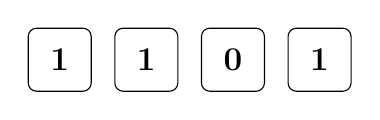
\begin{tikzpicture}[baseline=-0.5ex, every node/.style={align=center}]
    \foreach \digit [count=\i from 0] in {1, 1, 0, 1} {
        \node[draw, minimum width=0.8cm, minimum height=0.8cm, rounded corners=3pt] (tub\i) at (\i*1.1, 0) {\large $\mathbf{\digit}$};
    }
\end{tikzpicture}
\end{center}

Nun schreiben wir unter die einzelnen Zahlen die 2-er Potenzen:

\begin{center}
$1101 = $
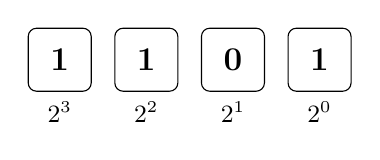
\begin{tikzpicture}[baseline=-0.5ex, every node/.style={align=center}]
    \foreach \digit/\power [count=\i from 0] in {1/2^3, 1/2^2, 0/2^1, 1/2^0} {
        \node[draw, minimum width=0.8cm, minimum height=0.8cm, rounded corners=3pt] (tub\i) at (\i*1.1, 0) {\large $\mathbf{\digit}$};
        \node[anchor=north, font=\small] at (tub\i.south) {$\power$};
    }
\end{tikzpicture}
\end{center}

Jetzt schreiben wir darunter das Produkt der Ziffern mit den 2-er Potenzen und summieren diese:

\begin{center}
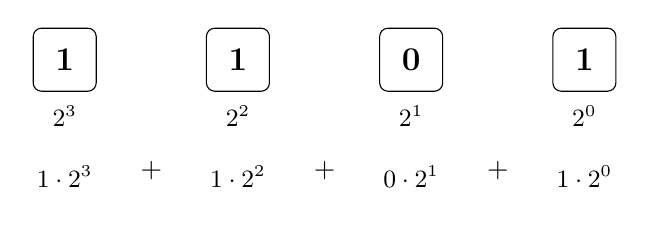
\begin{tikzpicture}[baseline=(box0.base), every node/.style={align=center}]
    \foreach \digit/\power/\prod [count=\i from 0] in {
        1 / 2^3 / 1 \cdot 2^3,
        1 / 2^2 / 1 \cdot 2^2,
        0 / 2^1 / 0 \cdot 2^1,
        1 / 2^0 / 1 \cdot 2^0
    } {
        \pgfmathsetmacro{\xpos}{\i*2.2}
        \node[draw, minimum width=0.8cm, minimum height=0.8cm, rounded corners=3pt] (box\i) at (\xpos, 0) {\large $\mathbf{\digit}$};
        \node[anchor=north, font=\small] (pow\i) at ([yshift=-0.05cm]box\i.south) {$\power$};
        \node[anchor=north, font=\small] (prod\i) at ([yshift=-0.25cm]pow\i.south) {$\prod$};
        \ifnum\i<3
            \node[anchor=base] at ({\xpos + 1.1}, {-0.8 - 0.7}) {$+$};
        \fi
    }
\end{tikzpicture}
\end{center}

Zum Schluss rechnen wir das Ganze aus:

\begin{center}
\begin{align*}
  &\phantom{= } 1 \cdot 2^3 + 1 \cdot 2^2 + 0 \cdot 2^1 + 1 \cdot 2^0 \\
  &= 1 \cdot 8 + 1 \cdot 4 + 0 \cdot 2 + 1 \cdot 1 \\
  &= 8 + 4 + 0 + 1 \\
  &= 13
\end{align*}
\end{center}


Schauen wir uns als nächstes eine größere Zahl an, zum Beispiel \textbf{11010110}. Auch hier wenden wir exakt dasselbe Prinzip an:

\begin{center}
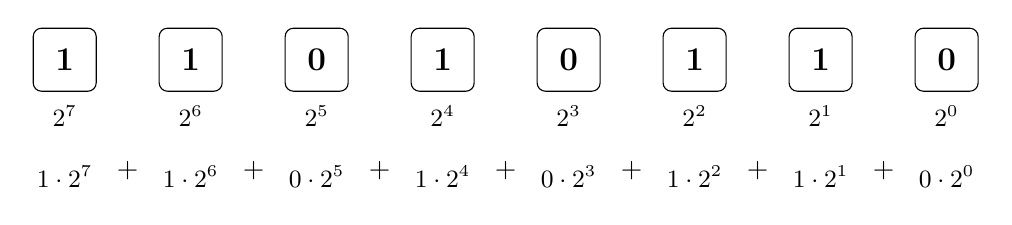
\begin{tikzpicture}[baseline=(box0.base), every node/.style={align=center}]
    % Schleife für die 7 Spalten der Zahl 8305710 (Ziffer / Potenz / Produkt)
    \foreach \digit/\power/\prod [count=\i from 0] in {
        1 / 2^7 / 1 \cdot 2^7,
        1 / 2^6 / 1 \cdot 2^6,
        0 / 2^5 / 0 \cdot 2^5,
        1 / 2^4 / 1 \cdot 2^4,
        0 / 2^3 / 0 \cdot 2^3,
        1 / 2^2 / 1 \cdot 2^2,
        1 / 2^1 / 1 \cdot 2^1,
        0 / 2^0 / 0 \cdot 2^0
    } {
        % X-Position für jede Spalte berechnen (Abstand 2.2cm)
        \pgfmathsetmacro{\xpos}{\i*1.6}

        % 1. Zeile: Die Wanne mit der Ziffer darin
        \node[draw, minimum width=0.8cm, minimum height=0.8cm, rounded corners=3pt] (box\i) at (\xpos, 0) {\large $\mathbf{\digit}$};

        % 2. Zeile: Die Zehnerpotenz direkt darunter
        \node[anchor=north, font=\small] (pow\i) at ([yshift=-0.05cm]box\i.south) {$\power$};

        % 3. Zeile: Das Produkt direkt unter der Potenz
        \node[anchor=north, font=\small] (prod\i) at ([yshift=-0.25cm]pow\i.south) {$\prod$};

        % Pluszeichen in den Lücken zwischen den Produkten (bis zum vorletzten Element, hier i < 6)
        \ifnum\i<7
            \node[anchor=base] at ({\xpos + 0.8}, {-0.8 - 0.7}) {$+$};
        \fi
    }
\end{tikzpicture}
\end{center}

Zum Schluss rechnen wir das Ganze aus:

\begin{center}
\begin{align*}
  &\phantom{= } 1 \cdot 2^7 +1 \cdot 2^6 + 0 \cdot 2^5 + 1 \cdot 2^4 + 0 \cdot 2^3 + 1 \cdot 2^2 + 1 \cdot 2^1 + 0 \cdot 2^0 \\
  &= 1 \cdot 128 + 1 \cdot 64 + 0 \cdot 32 + 1 \cdot 16 + 0 \cdot 8 + 1 \cdot 4 + 1 \cdot 2 + 0 \cdot 1 \\
  &= 128 + 64 + 0 + 16 + 0 + 4 + 2 + 0 \\
  &= 214
\end{align*}
\end{center}
\end{document}
